\section{Introduction}

In Chapter \ref{ch:constraining_optimization} we looked at enforcing properties of deep networks by constraining the optimization process. In this chapter we focus on the similar problem of deriving guarantees on the properties of deep networks by analysing the optimized artefact. For example, just as we previously ensured the predictions of deep networks in convex hulls around training points in Section \ref{sec:instance_robustness}, in this chapter we will show how to guarantee predictions in regions of the input space. This broad field of guaranteeing deep network behaviour through mathematical arguments is known as formal verification.

\section{Predictions}

\begin{theorem}\label{thm:prediction_verification}
    Consider a binary classifier $f$ and let $\omega\in\Omega$ have vertices $\left\{\mathbf{v}_1,\dots,\mathbf{v}_p\right\}$. Then if $$\left\vert\sum_{j=1}^p\mathrm{sign}\left(\left\langle\left[W^{(L)}\right]_{1,\cdot},f^{(\ell-1)}\left(\mathbf{v}_j\right)\right\rangle+\left[b^{(L)}\right]_1\right)\right\vert=p,$$then $f$ makes the same classification prediction for every $\mathbf{x}\in\omega$. 
\end{theorem}

\begin{tproof}
    \TODO
\end{tproof}

\begin{remark}
    \begin{enumerate}
        \item[]
        \item Note the similarity between Theorem \ref{thm:prediction_verification} and Theorem \ref{thm:provable_instance_constraint}.
        \item From Theorem \ref{thm:prediction_verification}, it follows that it suffices to understand the predictions of the deep network at the vertices of a given region to make inferences on the predictions it will make for all points within the region $\omega$.
    \end{enumerate}
\end{remark}

\TODO
\begin{figure}
    \centering
    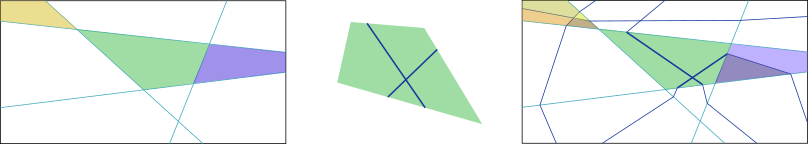
\includegraphics[width=0.8\linewidth]{drawings/iterative_partitioning_procedure.png}
    \caption{The training data is depicted as scatter points, colour-coded according to the class that they belong too. The highlighted regions correspond to regions for which it can be guaranteed that the deep network predicts the class associated to that colour.}
    \label{fig:prediction_verification}
\end{figure}

Typically, regions $\omega\in\Omega$ induced by $f:\mathbb{R}^d\to\mathbb{R}$ are bounded by on the order of $d$ vertices. Although it seems as though we can guarantee the behaviour of a deep network by only checking its behaviour on a relatively few number of determinable points, computing the points is computationally expensive. However, as shown in Section \ref{sec:splinecam}, this computations are tractable when we restrict ourselves to a two-dimensional slice of the input domain. If the input domain is two-dimensional, then we would be able to make statements such as the robustness of instances in our input domain.

\begin{example}
    Suppose that we have a deep network $f:\mathbb{R}^2\to\mathbb{R}$ comprising of four fully connected operators composed with ReLU non-linearities. We can train this deep network to perform two-class classification on a set of training data. Since $f$ is a continuous affine spline, it induces a partition of the input space. Let $P$ be a two-dimensional polytope encompassing the training data. Then using Algorithm \ref{alg:cycles} we can obtain the partition and thus the vertices bounding the regions of $\Omega$ intersecting $P$. We can then use Theorem \ref{thm:prediction_verification} to identify regions on which we can guarantee the predictions of our deep network, Figure \ref{fig:prediction_verification}. Of course, we can make $P$ arbitrarily larger to improve the strength of the inferred guarantees. However, this comes with additional computational costs as more regions $\omega$ would intersect $P$, resulting in the effects outlined in Proposition \ref{prop:complexity_splinecam}. For practical purposes, formal verification only really needs to be able to provide guarantees on likely inputs to our deep network. Clearly from observing the data in Figure \ref{fig:prediction_verification}, it is clear that $P$, and the verified region, captures a significant proportion of training data distribution.
\end{example}

In the case where our input domain has more than two-dimensions all is not lost, as certain properties of the input domain lie on two-dimensional subspaces; meaning we can verify predictions for specific properties in the input domain.

\begin{example}
    \begin{enumerate}
        \item[]
        \item Suppose that our deep network is receiving flattened images as its input. Then for an image $\mathbf{x}$, verifying predictions in the two-dimensional subspace spanned by $\mathbf{v}_1:=\frac{\mathbf{x}}{\Vert\mathbf{x}\Vert}$ and $\mathbf{v}_2=\text{gramschmidtvector}$ corresponds to verifying the predictions of the deep network as the brightness of the image $\mathbf{x}$ is varied.
        \item It has been shown that features of a deep network can correspond directions in input space of deep networks, Section \ref{sec:directions_as_units}. Therefore, verifying predictions in the two-dimensional spanned by these directions and an orthogonal direction corresponds to verifying the predictions of the deep network for inputs expressing this feature to various degrees.
    \end{enumerate}
\end{example}

\section{References}